% !TEX TS-program = pdflatex
% !TEX encoding = UTF-8 Unicode

% This is a simple template for a LaTeX document using the "article" class.
% See "book", "report", "letter" for other types of document.

\documentclass[11pt]{article} % use larger type; default would be 10pt

\usepackage[utf8]{inputenc} % set input encoding (not needed with XeLaTeX)


%%% PAGE DIMENSIONS
\usepackage{geometry} % to change the page dimensions
\geometry{a4paper} % or letterpaper (US) or a5paper or....


\usepackage{graphicx} % support the \includegraphics command and options

% \usepackage[parfill]{parskip} % Activate to begin paragraphs with an empty line rather than an indent

%%% PACKAGES
\usepackage{booktabs} % for much better looking tables
\usepackage{array} % for better arrays (eg matrices) in maths
\usepackage{paralist} % very flexible & customisable lists (eg. enumerate/itemize, etc.)
\usepackage{verbatim} % adds environment for commenting out blocks of text & for better verbatim
\usepackage{subfig} % make it possible to include more than one captioned figure/table in a single float
\usepackage{cite}

\usepackage{amsmath,amscd}
\usepackage{amssymb,array}
\usepackage{amsfonts,latexsym}
\usepackage{graphicx,subfig,wrapfig}
\usepackage{times}
\usepackage{psfrag,epsfig}
\usepackage{verbatim}
\usepackage{tabularx}
\usepackage[pagebackref=true,breaklinks=true,letterpaper=true,hidelinks,bookmarks=false]{hyperref}
\usepackage{ mathrsfs }
% These packages are all incorporated in the memoir class to one degree or another...

%%% HEADERS & FOOTERS
\usepackage{fancyhdr} % This should be set AFTER setting up the page geometry
\pagestyle{fancy} % options: empty , plain , fancy
\renewcommand{\headrulewidth}{0pt} % customise the layout...
\lhead{}\chead{}\rhead{}
\lfoot{}\cfoot{\thepage}\rfoot{}

%%% SECTION TITLE APPEARANCE
\usepackage{sectsty}
\allsectionsfont{\sffamily\mdseries\upshape} % (See the fntguide.pdf for font help)
% (This matches ConTeXt defaults)

%%% ToC (table of contents) APPEARANCE
\usepackage[nottoc,notlof,notlot]{tocbibind} % Put the bibliography in the ToC
\usepackage[titles,subfigure]{tocloft} % Alter the style of the Table of Contents
\renewcommand{\cftsecfont}{\rmfamily\mdseries\upshape}
\renewcommand{\cftsecpagefont}{\rmfamily\mdseries\upshape} % No bold!



\title{Models of the Neuron: Project 2 \\ Forward motion response inhibition of \emph{C. elegans} as a result of interneuron ablations}
\author{Greg Kiar}
%\date{} % Activate to display a given date or no date (if empty),
         % otherwise the current date is printed 

\begin{document}
\maketitle

\section{Introduction}

Connectomics is a young and burgeoning field which aims to produce connectomes, complete neural connectivity maps, for living organisms. The \emph{Caenorhabditis elegans} (\emph{C. elegans}) roundworm is studied in this field because of its simple and small nervous system consisting of only $302$ neurons \cite{Sulston1977,White1986,Dunn2003, Chen2006}. Due to the lack of both computational resources and fundamental knowledge, the human nervous system is impractical to model. However, researchers are able to model \emph{C. elegans} by exploiting the simplicity of its complete neural network \cite{Iwasaki2006, Iwasaki2004, Dunn2003, Wicks1996a}. One such modeling paper of interest, written by Kunert et al.\cite{Kunert2014}, studies the effect of AVA and AVB interneurons on forward motor response of \emph{C. elegans}. Kunert et al. study the effect of specific interneurons on signal transmission to the motor neurons by ablating AVA and ABA neurons in a pairwise fashion (left and right simultaneously) \cite{Kunert2014}. This paper aims to recreate the model implemented in \cite{Kunert2014} to scale, and expand upon the reported ablation and motor response dynamic results.

The work performed in this study allows for better insight to be gained on the topic of motor control in \emph{C. elegans}. This project will study the effect of individual neuron ablation within the AVAL, AVAR, and AVBL, AVBR sets on forward motor response. Posing this question in the context of \cite{Kunert2014} is analogous to presenting a large graph solution where previously only a small graph solution had been explored. Expanding knowledge in this field can lead to better understanding of and possibly suggest mechanisms for synaptic plasticity when non-pairwise ablations occur in the \emph{C. elegans} nervous system. A secondary objective of this study is to determine whether a partial network model for \emph{C. elegans}, consisting only of neurons of immediate relevance, can be studied and produce equivalent results to that of a complete network. For documentation of all code pertaining to this study, please see the attached files.

\section{Background and Outline}
In Kunert et al. \cite{Kunert2014} a network is constructed of $279$ neurons of \emph{C. elegans} based on known connectome data \cite{Varshney2011}. Only $279$ somatic neurons of the $302$ total neurons \cite{Sulston1977} were included in the model; those exclused were done so by the prescription of \cite{Varshney2011}. The neurons not included made up a set that comprised of pharyngeal and isolate (with no connections) neurons \cite{Varshney2011}. Kunert et al. observed the relationships between forward motor activation based on the DB, DD, VB, and VD motor neurons. The forward motion was observed with respect to the ablation of two regions of interneurons AVA and AVB \cite{Kunert 2014} which are known to contribute to forward movement, much like was done experimentally in \cite{Chalfie1985}. The findings of this paper showed that the full ablation of the AVB interneuron resulted in inhibited forward motor response, whereas ablation of AVA did not have a significant effect.

Effort was made here to reproduce this result with a simplified neural network and take the research question a step further. Before a research question could be posed, a model equivalent to that used by Kunert et al. needed to be produced. In order to accomplish this within the scope of the course, a partial network was be constructed. Initially, a single neuron was modelled using the single-compartment model \cite{Wicks1996a} as it was implemented in \cite{Kunert2014}. Once the results of this were verified against the published findings, a small network was constructed based on published physiological data about the \emph{C. elegans} (see: \cite{Wicks1996a, Varshney2011, Sulston1977, Oshio2003}). The subset selected was chosen based on the neurons which were most central to the aims of this project (discussed in detail later on). A simplified network model inherently has fewer signals and inputs to each node, which will contribute to a source of error in the model. This was mitigated by adding additional random input currents to each neuron in the model.

Using the simplified network and neuron structure as implemented above, this work aims to assess the forward-controlling motor neuron response of \emph{C. elegans} for interneuron single and pair ablation, where previously only pairwise ablations were studied \cite{Kunert2014}. AVA and AVB neuron sets were ablated both individually and in sets, meaning that their synaptic and gap junctions were removed from the network. This work aims to determine if the AVA and AVB neuron pairs together are required for effective signal to motor transduction, or if a portion of each interneuron set would result in significant inhibition of motor response as was seen with compelte AVB ablation \cite{Kunert2014, Chalfie1985}. This work identifies whether a simplified model as described can be used as a tool through which more specific ablation testing can be done at lower computational cost, and whether the findings presented by Kunert et al. may be incomplete regarding the cause of their observed forward motor inhibition.

\section{Methods}

Before modifications could be made and the work expanded upon, the initial model implemented by Kunert et al. needed to be replicated. The model was created for a single neuron and the resulting behaviour compared to the results presented in \cite{Kunert2014}. The single neuron model was then integrated into a small network consisting of the neurons within the neighborhood of the AVA and AVB interneurons. The network dynamics were then tested with the ablation of individual interneurons within the created network.

\subsection{Single Neuron}
The neuron model which was used in \cite{Kunert2014} and accurately represents the \emph{C. elegans} neuron behaviour is the so-called "single-compartment membrane" equation \cite{Kunert2014, Wicks1996a}. This model is able to accurately represent the neurons in \emph{C. elegans} because they are essentially isopotential, meaning that they have the same potential uniformly distributed across each neuron \cite{Goodman1998}. The equations used in this model are given by \cite{Kunert2014}:
\begin{align}
C \dot{V} &= -G_c(V_i - E_{cell}) - I_i^{Gap}(\vec{V}) - I_i^{Syn}(\vec{V}) + I_i^{Ext}
\end{align}
Where $C$ is the membrane capacitance, $G_c$ is the membrane leakage conductance, and $E_{cell}$ is the membrane leakage potential. $I_i^{Ext}$ is the applied external current to the neuron. $I_i^{Gap}(\vec{V})$ and $I_i^{Syn}(\vec{V})$ are gap and synaptic currents, respectively, from interactions with other neurons and are defined by:
\begin{align}
I_i^{Gap}(\vec{V}) &= \sum_j G_{ij}^g(V_i - V_j) \\
I_i^{Syn}(\vec{V}) &= \sum_j G_{ij}^s s_j(V_i - E_j)
\end{align}
Where $G_i^g$ is the total gap conductance, $G_i^s$ is the synaptic conductance, $E_j$ is the reversal potential of the synapse, and $s_j$ is the synaptic activation defined by:
\begin{align} \label{eq:sdot}
\dot{s}_j &= a_r \phi (V_j; \beta, V_{th})(1-s_j) - a_d s_j
\end{align}
With $a_r$ and $a_d$ as rate constants, and $\phi$ is a squashing function defined as:
\begin{align} 
\phi (V_j; \beta, V_{th}) &= \frac{1}{1+ e^{-\beta(V_j - V_{th})}}
\end{align}
Where $\beta$ adjusts the width of this function and $V_{th}$ is the Thevenin equivalent potential \cite{Wicks1996a}. The parameters used in creating this model were consistent with those presented in \cite{Kunert2014} with the exception of the reverse rate constant, $a_d$. The value presented was $a_d=5$; this value caused the system as implemented above to be unstable even in the presence of no input (i.e. Equation \ref{eq:sdot} diverged to infinity when started slightly off of equilibrium). As a result, it was interpretted here that this value was mistakenly reported due to a typing error and the value of $a_d = 0.5$ was used.

Shown in Figure \ref{fig:f1} is the implementation of this model for a single, isolate neuron. It can be seen that the neuron here matches the single neuron implementation as can be seen in FIG. 2(b) \cite{Kunert2014}. By comparing the plots, it can be observed that the rise and decay times of the membrane potential curves correspond to one another, as well as the range over which the voltage changes with this applied current.
\begin{figure}[h!]
\begin{center}
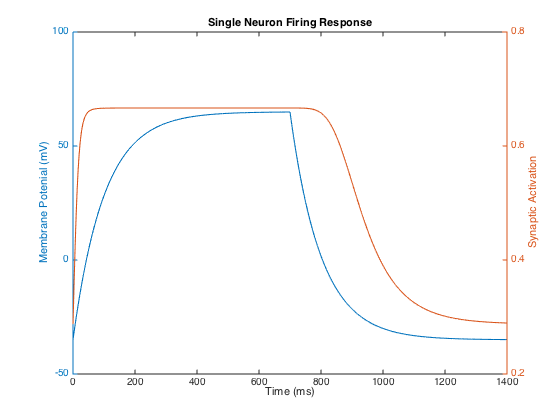
\includegraphics[scale=0.4]{motn_fig1.png} \caption[h1]{Single-compartment model response for a single, isolated neuron. Due to isolation, the synaptic and gap currents, $I^g(\vec{V}) = I^s(\vec{V}) = 0$. The external current applied was in $10 pA$ in amplitude and was applied from $t=0\to750 ms$. The blue trace shows the potential as a result of this applied current, and the orange trace shows the synaptic activation based on this potential. It is worth noting that due to the structure of the equation, in an isolated neuron, the synaptic activation does not play a role in the membrane potential.} \label{fig:f1} \end{center}
\end{figure}  

%\newpage
\subsection{Small Network}
A network of neurons needed to be constructed to test the overall system dynamics once the single neuron dynamics were verified. Since the neural network for \emph{C. elegans} consists of 302 neurons with several thousand documented connections \cite{Varshney2011}, a subset of this network was selected to be modeled. Kunert et al. studied the effect of ablation of AVB and AVA interneurons on forward motor response, particularly that of the DB, DD, VB, VD motor neurons \cite{Kunert2014}. With that in mind, the subset selected to be modeled, as shown in Figure \ref{fig:f2}, consisted of all of these neuron groups of interest. For simplicity of the model, neurons within each category, for instance  AVAL and AVAR, were grouped into a single node, AVA, at this stage of the model.
\begin{figure}[h!]
\begin{center}
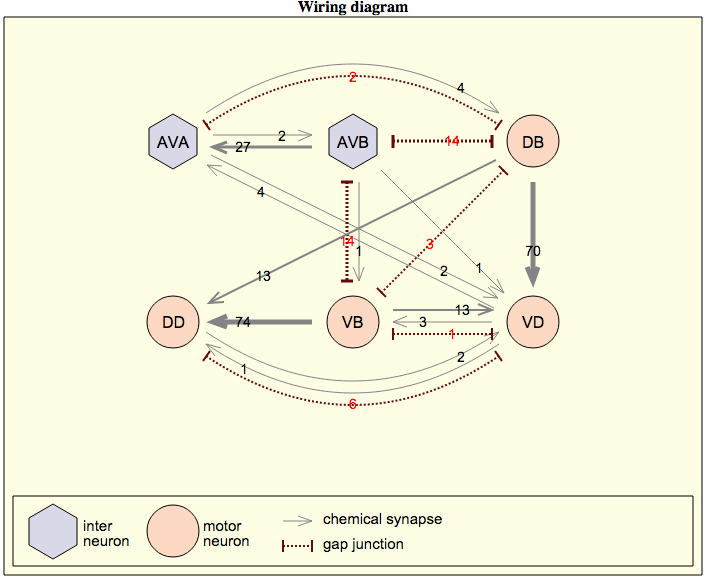
\includegraphics[scale=0.35]{motn_fig2.png} \caption[h2]{Wiring diagram for the selected subset of neurons constructed. The graphic of this network was constructed using the Database for Synaptic Connectivity of \emph{C. elegans} for Computation \cite{Oshio2003}. The numbers over each line describe the number of a given type of connection between two nodes. Due to the linear nature of the differential equations and neuron model used, the number of connections between nodes were taken to be weight vectors, and the corresponding signals were scaled accordingly.} \label{fig:f2} \end{center}
\end{figure}
Though the connectome of \emph{C. elegans} is largely known, synaptic polarities of these connections are less understood \cite{Rakowski2013}. Because of this, the polarity of all of the synapses modeled was not implicit with the connections themselves. Based on previous research showing responses to neuron connectivity and ablation \cite{Kunert2014, Chalfie1985, White1986, Chen2006} and public resources \cite{Altun2003, Oshio2003} documenting the purpose of specific connections within the \emph{C. elegans} connectome, educated guesses were made as to the polarity of each synapse for the purposes of this paper. From the findings presented in \cite{Chalfie1985}, where AVA and AVB ablation inhibit motor response in the DB, DD, VB, and VD motorneurons, their outgoing synapses were set to be excitatory. Due to the description of the function of the motor neurons in question as found in \cite{Altun2003}, the motor neuron synapses were set to be excitatory between the same class of neurons (i.e. DB to VB) but inhibitory across classes (i.e. DB to DD). The snapses feeding back from the motorn neurons to the interneurons were set to be inhibitory. As mentioned above, this directed network was created through inference and an educated guess as an approximation due to lack of conclusive evidence stating the polarity of the synaptic junctions. Figure \ref{fig:f3} shows the assigned polarity for each set of created synapses. 

Since the network simulated was an incomplete simulation of the entire \emph{C. elegans} nervous system, random noise in the form of input current was added to each channel to simulate neural activity through the not-modeled synapses. It was noted that this was an unideal way to model larger network dynamics, and discussion regarding that will follow.
\begin{figure}[h!]
\begin{center}
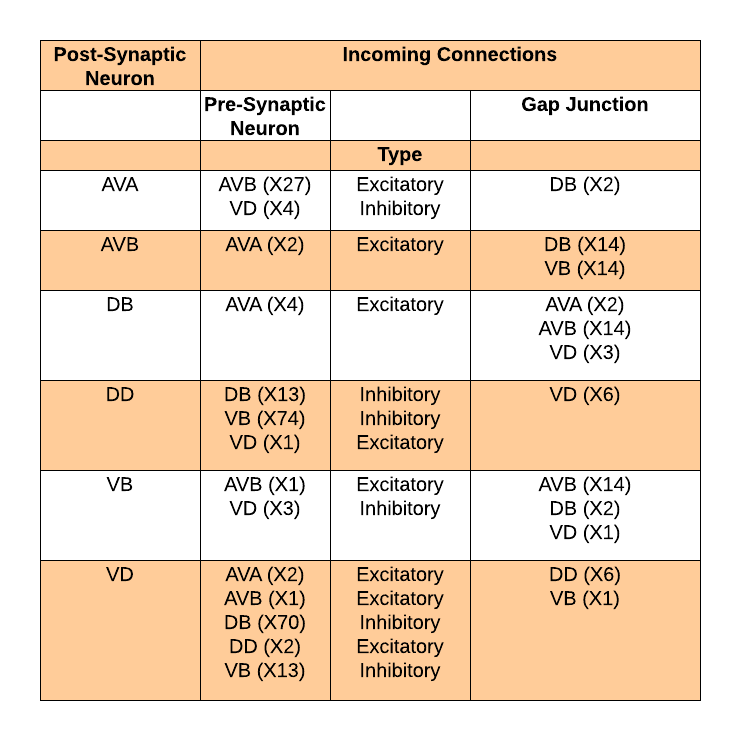
\includegraphics[scale=0.63]{motn_fig3.png} \caption[h3]{Polarity assignment of synaptic junctions between all combinations of interneurons and motor neurons present in the network created. Polarities assigned were based on prior knowledge \cite{White1986, Chen2006} of synaptic effects of neurons on one another, and physiological information of the behaviour of each neuron \cite{Altun2003, Chalfie1985}.} \label{fig:f3} \end{center}
\begin{center}
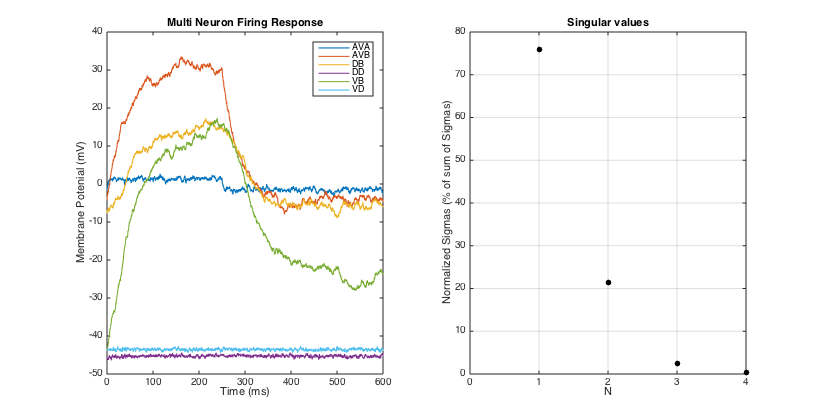
\includegraphics[scale=0.45]{motn_fig4.png} \caption[h4]{Left: Dynamics of each modelled neuron group for applied current on the AVA and AVB neurons. It can be seen that the four motor neuron categories have varying responses and equilibrium states from one another. This finding is consistent with results presented in \cite{Kunert2014} as well as behavioural data of \emph{C. elegans} \cite{Iwasaki2004} which states that the VB and DB motor neurons are involved in forward movement, whereas DD and VD are not. The neuron responses corresponded to this activation for forward movement. Right: Computed from Equation \ref{eq:svd}, are the singular values for the network. Much like is seen in Kunert et al., the first two modes are heavily dominant in this system \cite{Kunert2014}, again illustrating that the DB and VB motor neurons dominated the response.} \label{fig:f4} \end{center}
\end{figure}
\\

The dynamics of the network produced are shown in Figure \ref{fig:f4} for an input current as shown above for a single neuron. The current stimulating this model was solely applied to the AVB and AVA interneurons; this was done to simulate the "down-stream" effect on the motor neurons, much like would occur in a full neural network in which a motor signal is being transmitted. In order to analyze the behaviour of this network, the singular value decomposition (SVD) of the voltages was done and the singular values were observed as follows \cite{Kunert2014}:
\begin{align} \label{eq:svd}
V &= \begin{bmatrix}V_M(t_0) & V_M(t_1) & \hdots & V_M(T)\end{bmatrix} = U \Sigma V^T 
\end{align}
Where $V_M(t)$ is defined as a snapshot of all of the motor neuron voltages for each point in time. From here, with $4$ motor neurons, $\Sigma$ is truncated down into the first $4$ diagonal values (the matrix is sparse) and plotted in Figure \ref{fig:f4}. We can see a clear dominance of the first two modes of the network, with $\sigma_{1,2} \gg \sigma_{3,4}$. What this finding suggests is that the response of the network is dominated by two time-dependent voltage responses \cite{Kunert2014}.

\clearpage
\subsection{Network Ablations}
Testing the effect of partial ablations on motor response requires knowledge of connections to each of the neurons within the AVA and AVB classes. The connection data obtained from \cite{Oshio2003} provides the AVB and AVA neurons and their connections can be decomposed into left and right components, serving this purpose. In order to test the effect of partial and complete ablation on the network, the subset of connections pertaining to each AVAL, AVAR, AVBL, AVBR, as well as the total AVA and AVB neuron categories were sequentially ablated. The neurons were ablated by adjusting the linear weights imposed by Figure \ref{fig:f2} above to effectively remove the connections to the neuron under inspection.
\section{Ablation Results}
Shown in Figure \ref{fig:f5} is the result of ablating different combinations of the AVAL, AVAR, AVBL, and AVBR interneurons. For comparison with \cite{Kunert2014}, AVA and AVB neurons were also fully ablated. From data obtained in the non ablation network test, as shown in Figure \ref{fig:f4}, the first two singular values (representing forward motor response) were $75.9\%$ and $21.3\%$ of the sum of squared singular values for the system. It can be seen that the AVA ablation had a minor impact on forward motor response, but the singular values remained similar at values of $79.5\%$ and $15.8\%$. However, when looked at the AVB ablation response we can see that there is a significant change in the singular values, which became $89.2\%$ and $7.38\%$. These findings qualitatively match those presented in \cite{Kunert2014}.
\begin{figure}[h!]
\begin{center}
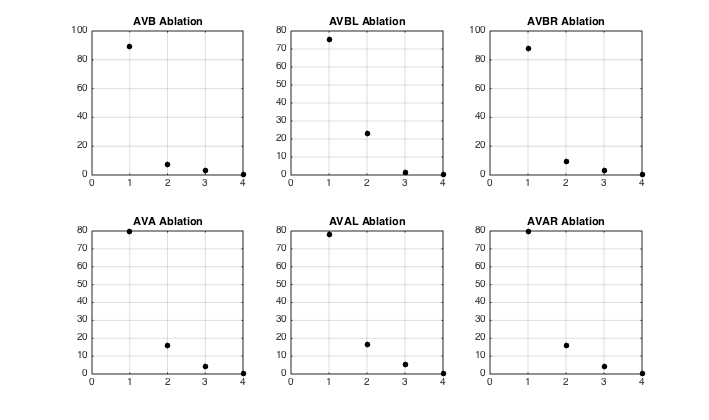
\includegraphics[scale=0.48]{motn_fig5.png} \caption[h4]{Network ablations for partial and complete AVA and AVB sets. AVA shows little change in singular values/mode of response compared to the unablated network; for all sets of ablations tested. AVB however shows significant inhibition when both neurons are ablated. There is also significant inhibition when the AVBR interneuron is the only ablated neuron.} \label{fig:f5} \end{center}
\end{figure} \\
Looking now at the indivual neuron ablations, we can see both AVAL and AVAR ablations have minimal impact on the motor response. This conclusion is consistent as the combination of both ablations also failed to inhibit forward motor activity. When we look at the AVBL and AVBR ablations we can, unlike the case with AVAL and AVAR, see a distinct difference between their singular values. In the case of AVBL ablation the singular values were $75.0\%$ and $23.0\%$, which are similar to that of the unablated network. The AVBR singular values after ablation are significantly different, $87.7\%$ and $9.16\%$, which shows that the AVBR interneuron does play a role in this overall observed ablation effect of AVB neurons. This finding suggests that inhibited forward movement due to AVB ablation as was observed \cite{Chalfie1985} and modeled \cite{Kunert2014} could be more specifically due to AVBR ablation, with AVBL left untouched. 
\section{Conclusion}
This study created a simplified neural network of \emph{C. elegans} with the aim of reproducing and exploring motor inhibition caused by interneuron ablation. It was found that the network that was produced yielded similar results to that of the model paper, Kunert et al. 2014. The results presented here suggest that not only does AVB ablation inhibit forward motor response in \emph{C. elegans}, but more specifically the AVBR interneuron is almost solely responsible for this result. This result however is not conclusive due to the nature of the model produced, and the approximations made in order to simplify it from the full \emph{C. elegans} connectome.

In future work, this project could be expanded and improved upon by increasing the level of sophistication within the model. Here, random currents were added as noise to each input to simulate the rest of a network, which is an simplistic way to simulate the remainder of a circuit. Using stochastic methods \cite{Iwasaki2006}, a more accurate representation of the rest of the \emph{C. elegans} connectome could be approximated. Another way in which this model could be improved is by adding more neuron types to the model. With a larger subset of the network, the approximation would inherently be closer.

This study suggests evidence that the findings presented by Chalfie et. al, 1985, and reproduced in a model by Kunert et al. 2014, are correct but incomplete. Here we suggest and defend the more focused hypothesis that the AVBR interneuron specifically is largely responsible for forward motion in \emph{C. elegans}. This result agrees with previous findings, but provides a greater resolution through which the solution is expressed.

\section{Acknowledgements}
Thank you, Dr. Young, for a very fun and interesting class. I came in with practically no neurophsyiology knowledge, and left with at least double that. I learned a great deal this semester and in this project in particular. All the best.
\clearpage
\bibliography{mine}{}
\bibliographystyle{plain}

\end{document}
